\newpage
\begin{center}
    \Huge{\textbf{\underline{Chapter 5: Fixed-Point Mehtod}}}
\end{center}

\vspace{0.77cm}
\setcounter{section}{0}

\begin{prettyBox}{Implementation}{myblue}
\begin{itemize}
\item \texttt{phi\_function(x)}: Computes the value of the function \( \varphi(x) \) at a
given point \( x_n \), following the recurrence relation:  
          \[
          x_{n+1} = \varphi(x_n)
          \]
\item \texttt{ErrorEstimation(a, b)}: Estimates the error at iteration \(n\) for a given 
contraction factor \( k \in ]0,1[\), using the formula:  
          \[
          \dfrac{k^n}{1-k} \cdot |x_0 - x_1|
          \]

    \item \texttt{eps}: Defines the error tolerance \( \epsilon \), determining the stopping
    criterion.

    \item \texttt{max\_iter}: Specifies the maximum number of iterations allowed in the 
fixed-point algorithm.

\item \texttt{Fixed\_Point(eps, k, x\_0, function, max\_iter=100)}: Computes the root of \( f(x) \) with the fixed-point method with the  
its corresponding \( \varphi(x) \) and contraction factor \( k \), starting from an
initial \( x_0 \) with a tolerance \( \epsilon \) and the maximum number of iterations max\_iter (default: 100).
\end{itemize}
\end{prettyBox}
\vspace{0.5cm}
\textbf{\underline{Code}}\\[0.05cm]
\lstinputlisting[style=pythonstyle]{Chapters/Code/FIX/fix.py}

\newpage
\textbf{\underline{Example}}\\[0.1cm]
\lstinputlisting[style=pythonstyle]{Chapters/Code/FIX/ex1.py}

\vspace{0.5cm}

\begin{center}
    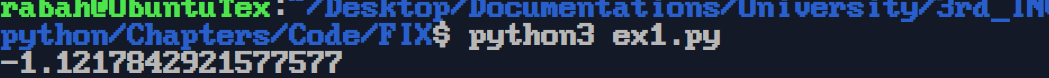
\includegraphics[width = 0.9\textwidth]{Chapters/ScreenShot/FIX/fix.png}
\end{center}

